\section{Mehrdimensionale Analysis}
  \subsection{Partielle Ableitung}
  \begin{definition}
    $f(x)$ heißt in $x^* \in \R^d$ nach der $j-ten$ Koordinate $x_j$ partiell diffbar, falls der Grenzwert
    \begin{equation}
      \frac{\partial f}{\partial x_j}(x^*) = \lim\limits_{t\rightarrow 0} \frac{f(x^* + t e_j) - f(x^*)}{t}
    \end{equation}
    existiert bzw. falls $\tilde{f}_j(x_j)$ in $x_j$ diffbar ist. $\frac{\partial f}{\partial x_j}(x^*)$ heißt die partielle Ableitung von $f$. 
  \end{definition}
  \begin{bem}
    Alternative Schreibweisen:
    \begin{equation}
      \frac{\partial f}{\partial x_j} = \frac{partial}{\partial x_j} f = \partial_{x_j} f = D_j f  = f_{x_j} = ...
    \end{equation}
  \end{bem}
  \begin{definition}
    Allgemein: n-te partielle Anleitung:
    \begin{equation}
      \frac{\diffp^2f}{\diffp x_k \diffp x_j} = \frac{\diffp f}{\diffp x_k}\left(\frac{\diffp f}{\diffp x_k} \right)
    \end{equation}
  \end{definition}
  
  \subsubsection{Gradient und Nabla Operator}
  \begin{definition}
    Der Zeilenvektor
    \begin{equation}
      \grad f(x^*) = \left( \dfp{f}{x_1}(x^*), ..., \dfp{f}{x_d}(x^*)\right)
    \end{equation}
    heißt der Gradient von $f$ in $x^*$. Es gilt weiter:
    \begin{equation}
      \nabla f(x^*) = (\grad f(x^*))^T
    \end{equation}
    Der eingeführte Operator heißt Nabla-Operator.
  \end{definition}
  \begin{satz}
    Sei $f:\R^d \rightarrow \R$ diffbar, dann gilt:
    \begin{itemize}
      \item[a) ] Der Gradientenvektor $\nabla f(x^*)$ steht senkrecht auf der Niveaumenge $N_{x^*} = \lbrace x \in \R^d: f(x) = f(x^*)\rbrace$
      \item[b) ] $\nabla f(x^*)$ gibt die Richtung des steilsten Anstiegs von $f(x)$ im Punkt $x^*$ an.
    \end{itemize}
  \end{satz}
  \begin{bem}
    Es gilt weiterhin:
    \begin{align}
      \grad(\alpha f + \beta g) &= \alpha \grad f + \beta \grad f, \qquad \alpha, \beta \in \R    \\  
      \grad (f\cdot g) &= f \cdot \grad g + g \cdot \grad f
    \end{align}
  \end{bem}
  
  \subsubsection{Jacobi Matrix}
  \begin{definition}
    Die Matrix der ersten Ableitung heißt die Jacobi Matrix. 
    \begin{equation}
      Jf = \left(\begin{array}{c c c}
      \dfp{f_1}{x_1} & \dots  & \dfp{f_1}{x_d} \\
      \vdots         & \ddots & \vdots         \\
      \dfp{f_m}{x_1} & \dots  & \dfp{f_m}{x_d} \end{array}\right)
    \end{equation}
  \end{definition}
  
  \subsection{Richtungsableitung}
  \begin{definition}
    Sei $f: \R^d \rightarrow \R$. Für $x^* \in \R^d$ und $v \in \R^d _{/ \lbrace 0 \rbrace}$ heißt
    \begin{equation}
      D_v f(x^*) = \lim\limits_{t\rightarrow 0} \frac{f(x^* +tv)-f(x^*)}{t}
    \end{equation}
    die Richtungsableitung von $f$ in $x^*$ in Richtung $v$. (Andere Schreibweise: $\dfp{f}{v})$
  \end{definition}
  Wenn alle Ableitungen existieren gilt:
  \begin{equation}
    D_v f = \grad f \cdot v
  \end{equation}
  \begin{bem}
    Der Gradient zeigt dabei selbst in Richtung des steilsten Anstiegs.
  \end{bem}
  
  \begin{satz}
    Ist $f: D\rightarrow \R$ mit $D \subset \R^d$ offen in einer Umgebung von $x^* \in D$ partiell diffbar und sind die partiellen Ableitungen dort beschränkt, dann ist $f$ stetig in $x^*$.
  \end{satz}
  
  \begin{satz}
    Existieren in einer Umgebung von $x^*$ alle partiellen Ableitungen und sind dann stetig in $x^*$, so ist $f$ diffbar in $x^*$. Allgemein gilt, existieren alle partiellen Ableitungen bis zur Ordnung $k$ und sind diese stetig, so ist $f \in C^k$, d.h. $k-fach$ stetig diffbar.
  \end{satz}
  
  \begin{bem}
    Folgerung: Alle Polynome, alle sin, cos, exp, ... Funktionen sind mehrdimensional diffbar.
  \end{bem}
  
  \begin{bem}
    Ist $f:\R^2 \rightarrow \R$ in einer Umgebung $U$ von $x^*$ partiell diffbar und sind diese in $x^*$ stetig, so ist $f$ diffbar in $x^*$.
  \end{bem}
  
  \subsection{Mehrdimensionale Kettenregel}
  \begin{satz}
  Sei $f: \R^n \rightarrow \R^m$ und $g: \R^m \rightarrow \R^d$. Sei $f$ in $x^*$ diffbar und $g$ in $y^* = f(x^*)$ diffbar. Dann ist $g \circ f$ in $x^*$ diffbar mit Jacobimatrix.
  \begin{equation}
    J(g \circ f) (x^*) = Jg(f(x^*)) \cdot Jf(x^*)\label{eq:mehrd_kettenr_jac}
  \end{equation}
  Somit gilt für $h(x) = g(f(x))$, dass
  \begin{equation}
    \dfp{z_{\colRed{k}}}{x_{\colBord{j}}} = \sum\limits_{\colBlue{i}} \dfp{z_{\colRed{k}}}{y_{\colBlue{i}}} \cdot \dfp{y_{\colBlue{i}}}{x_{\colBord{j}}}
  \end{equation}
  \end{satz}
  Vorgehen mit Jacobimatrix:\newline
  Es sei gegeben:
  \begin{align*}
    g: \R^2 \rightarrow \R ,\quad g(x,y) = f(x^2y, x+2y)
  \end{align*}
  \begin{flalign*}
    &\textbf{Schritt 1: } \text{Zur Übersichtlichkeit gegebenenfallsneue Funktionen definieren}&
  \end{flalign*}
  \vspace{-0.5cm}
  \begin{align*}
    q(x,y):= (x^2y, x+2y) \Rightarrow g(x,y) = f(q(x,y))
  \end{align*}
  \vspace{-0.5cm}
  \begin{flalign*}
    &\textbf{Schritt 2: } \text{Jacobimatrix der inneren Funktion aufstellen}&
  \end{flalign*}
  \vspace{-0.5cm}
  \begin{align*}
    Jq(x,y) = \left( \begin{array}{c c}
    2yx & x^2 \\
    1 & 2
    \end{array} \right)
  \end{align*}
  \vspace{-0.5cm}
  \begin{flalign*}
    &\textbf{Schritt 3: } \text{Jacobimatrix der äußeren Funktion in Abhängigkeit von der Inneren aufstellen}&
  \end{flalign*}
  \vspace{-0.5cm}
  \begin{align*}
    J_f(q(x,y)) = \left(\begin{array}{c c}
      \frac{\diffp f}{\diffp x}(q(x,y)) & \frac{\diffp f}{\diffp y} (q(x,y))
    \end{array}\right)
  \end{align*}
   \vspace{-0.5cm}
  \begin{flalign*}
    &\textbf{Schritt 4: } \text{\eqref{eq:mehrd_kettenr_jac} anwenden}&
  \end{flalign*}
  \vspace{-0.5cm}
  \begin{align*}
    J_g(x,y) = J_f(q(x,y)) \cdot J_q(x,y) = \left(\begin{array}{c c}
      \frac{\diffp f}{\diffp x}(q(x,y)) & \frac{\diffp f}{\diffp y} (q(x,y))
    \end{array}\right) \cdot
    \left( \begin{array}{c c}
    2yx & x^2 \\
    1 & 2
    \end{array} \right)
  \end{align*}  \vspace{-0.5cm}
  \begin{flalign*}
    &\textbf{Schritt 5: } \text{Ausmultiplizieren}&
  \end{flalign*}
  \vspace{-0.5cm}
  \begin{align*}
    J_g(x,y) &= 
    \left(
    \begin{array}{c c}
      2yx \frac{\diffp f}{\diffp x}(q(x,y)) + \frac{\diffp f}{\diffp y} (q(x,y)) & x^2 \frac{\diffp f}{\diffp x}(q(x,y)) + 2 \frac{\diffp f}{\diffp y (q(x,y))}
    \end{array}
    \right)\\
    \Rightarrow \frac{\diffp g}{\diffp x} (x,y) &= 2yx \frac{\diffp f}{\diffp x}(q(x,y)) + \frac{\diffp f}{\diffp y} (q(x,y)) \qquad \frac{\diffp g}{\diffp y} = x^2 \frac{\diffp f}{\diffp x}(q(x,y)) + 2 \frac{\diffp f}{\diffp y (q(x,y))}
  \end{align*}  
  
  \subsection{Wichtige Operatoren}
  \subsubsection{Divergenz}
  \begin{align}
    f: \R^d \rightarrow \R^d, f = (f_1, ..., f_d), x = (x_1, ..., x_d) \nonumber \\
    \diverg f = \sum\limits_{j=1}{d} \dfp{f_j}{x_j} = \dfp{f_1}{x_1} + \dfp{f_2}{x_2} + ... + \dfp{f_d}{x_d}
  \end{align}
  \begin{bem}
   Die Divergenz ist die Spur der Jacobimatrix, also die Summe der Diagonalelemente.
  \end{bem}
  
  \subsubsection{Laplace-Operator}
  \begin{align}
    &\varphi: \R^d \rightarrow \R \nonumber \\
    &\laplace \varphi = \nabla \nabla \varphi= \sum\limits_{j=1}^d \frac{diffp^2 \varphi}{\diffp x_j^2} = \frac{\diffp^2 \varphi}{\diffp x_1^2} + ... + \frac{\diffp^2 \varphi}{\diffp x_d^2}
  \end{align}
  \begin{bem}
   Der Laplace Operator bildet die Spur der Hesse Matrix.
  \end{bem}
  
  \subsubsection{Rotation}
  \begin{align}
    f:\R^3 \rightarrow \R^3 \nonumber \\  
    \rot f = \left( \begin{array}{c}
    \displaystyle\dfp{f_3}{x_2} - \dfp{f_2}{x_3} \\
    \displaystyle\dfp{f_1}{x_3} - \dfp{f_3}{x_1} \\
    \displaystyle\dfp{f_2}{x_1} - \dfp{f_1}{x_2}
    \end{array} \right)
  \end{align}
  \begin{bem}
    Die Bestandteile der Rotation sind die Nebendiagonalelemente der Jacobimatrix. Die Rotation gibt an wie \enquote{schief} die Jacobimatrix ist.
  \end{bem}    

  
  \subsection{Lemma von Schwarz}
  \begin{satz}
    Sei $f: \R^d \rightarrow \R$ eine $C^2$-Funktion, so gilt für alle $i,j \in \lbrace 1, ..., d\rbrace$:
    \begin{equation}
      \frac{\diffp^2 f}{\diffp x_i \diffp x_j} = \frac{\diffp^2 f}{\diffp x_j \diffp x_i}
    \end{equation}
  \end{satz}
  \begin{bem}
    Allgemein: Ist $f \in C^k$, dann ist die Reihenfolge des Differezierens bis zur $k-ten$ Ordnung egal.
  \end{bem}
  
  \subsection{Taylorscher Satz}
  \subsubsection{Wiederholung eindimensionaler Taylorscher Satz}
  \begin{equation}
    T(f, x, x^*) = \sum\limits_{k= 0}^n \frac{f^{(k)}(x^*)}{k!} (x-x^*)^k
  \end{equation}
  \subsubsection{Mehrdimensionaler Mittelwertsatz}
  \begin{satz}
    Sei $f: \R^d \rightarrow \R$ (hier wichtig: $\R$, nicht $\R^m$, $m\geq 2$) diffbar. Dann gibt es ein $\Theta\in (0,1)$ mit 
    \begin{equation}
      f(b) - f(a) = \ubGreen{\in \R^d}{\grad f(a+\Theta (b-a))}\ubGreen{\in \R^d}{(b-a)}
    \end{equation}
  \end{satz}
  \begin{bem}
    Der MWS gilt nicht für vektorwertige Funktionen.
  \end{bem}
  
  \subsubsection{Mehrdimensionaler Taylorscher Satz}
  \begin{definition}
    Offen: Um jeden Punkt $x \in D$ lässt sich eine Kugel in $D$ legen mit $r < 0$.
  \end{definition}
  \begin{definition}
    Konvex: Zu $x, y \in D$ ist auch die Verbindungsstrecke in $D$.
  \end{definition}
      
  \begin{satz}
    Sei $f: D\rightarrow \R$ eine $C^{m+1}$ Funktion auf einer offenen und konvexen Menge $D \in \R^d$ und $x^* \in D$. Dann gilt:
    \begin{align}
    &f(x) = Tm(x, x^*) + Rm(x, x^*) \\
    \text{mit} \nonumber \\
    &Tm(x, x^*) = \sum\limits_{j=0}^{m} \sum\limits_{j_1+j_2+...+j_d = j} \frac{1}{j_1!j_2!...j_d!} (x_1 - x_1^*)^{j_1} ... (x_d - x_d^*)^{j_d} \frac{\diffp^m f(x^*)}{\diffp x_1^{j_1} ... \diffp x_d^{j_d}} &\\
    \text{und} \nonumber \\
    &Rm(x, x^*) = \sum\limits_{j_1+j_2+...+j_d = m+1} \frac{1}{j_1!j_2!...j_d!} (x_1 - x_1^*)^{j_1} ...\nonumber \\ 
    &\qquad \qquad \qquad \qquad \qquad \qquad \qquad \cdot(x_d - x_d^*)^{j_d} \frac{\diffp^m f(x^*)}{\diffp x_1^{j_1} ... \diffp x_d^{j_d}}(x^* + \Theta(x-x^*))
    \end{align}
  \end{satz}
  
  \begin{bem}
    Taylorpolynome sind lokal die beste Approximation.
    \begin{equation}
      T1(x, x^*) = f(x^*) + \dfp{f}{x_1}(x^*)(x_1-x_1^*) + ... + \dfp{f}{x_d}(x_d-x_d^*)
    \end{equation}
    ist die Tangentialebene an $x^*$.
  \end{bem}
  
  \begin{bem}
    Zum Berechnen der Taylorpolynome ist es oft einfacher bekannte 1-dim Taylorpolynome bzw. Taylorreihne zu verwenden. Es git dann:
    \begin{equation}
      Tm(f, x, x^*) = T_a(f_a, x, x^*) \cdot ... \cdot T_d(f_d, x, x^*)
    \end{equation}
    Wobei auch mehrere Dimensionen mit einer 1-dim Reihe substituiert werden können.
  \end{bem}
  
  \subsubsection{Wichtige 1-dim Reihen}
  \begin{itemize}
    \item Exponentialreihe:
    \begin{equation}
      e^x = \sum\limits_{k=0}^\infty \frac{x^k}{k!} \qquad \forall x \in \R
    \end{equation}
    \item Geometrische Reihe
    \begin{equation}
      \frac{1}{1-q} = \sum\limits_{k = 0}^\infty q^k \qquad |q| < 1
    \end{equation}
    \item Sinusreihe
    \begin{equation}
      sin(y) = \sum\limits_{k = 0}^\infty \frac{(-1)^k y^{2k+1}}{(2k+1)!} = y -\frac{1}{3!}y^3 + \frac{1}{5!}y^5 + ...
    \end{equation}
    \item Cosinusreihe
    \begin{equation}
      cos(y) = \sum\limits_{k = 0}^\infty = (-1)^k \frac{y^2k}{(2k)!} = 1 - \frac{1}{2}y^2 + \frac{1}{4!}y^4 + ...
    \end{equation}
  \end{itemize}
  
  \subsection{Mehrdimensionale Extremwertaufgaben}
  Im Folgenden sei $f: \R^d \rightarrow \R$. 
  \begin{satz}
    Besitzt $f = f(x)$ in einem Punkt $x^*$ ein lokales Extremum (d.h. Minimum oder Maximum), so gilt
    \begin{equation}
      \nabla f(x^*) = 0
    \end{equation}   
  \end{satz}
  \begin{bem}
    $\nabla f(x^*) = 0$ liefert häufig keine Extrema sondern Sattelpunkte (je höher die Raumdimension desto wahrscheinlicher, dass kein Extrema vorliegt).
  \end{bem}   
  $f$ um $x^*$ lässt sich besser verstehen in dem man das Taylorpolynom 2. Grades um $x^*$ betrachtet. Dieses lässt sich mit Hilfe der Hesse-Matrix folgendermaßen formulieren:
  \begin{equation}
    T2(x, x^*) = f(x^*) + \nabla f(x^*)^T(x-x^*) + \frac{1}{2}(x-x^*)^T Hf(x^*)(x-x^*)
  \end{equation}
  Vorgehen zur Bestimmung von $T_2$: \newline
  \begin{flalign*}
    &\textbf{Schritt 1: } \text{Gradient von $f$ bestimmen}&
  \end{flalign*}
  \vspace{-0.5cm}
   \begin{flalign*}
    &\textbf{Schritt 2: } \text{Hesse Matrix von $f$ bestimmen}&
  \end{flalign*}
  \vspace{-0.5cm}
   \begin{flalign*}
    &\textbf{Schritt 3: } \text{$x^*$ einsetzen und ausrechnen}&
  \end{flalign*}
  \subsubsection{Hesse Matrix}
  Die Hesse Matrix ist die Matrix der zweiten Ableitung.
  \begin{equation}
    Hf(x^*) = J(Jf(x^*)) = f''(x^*) = \left(\begin{array}{c c c} 
    \displaystyle \frac{\diffp^2f}{\diffp x_1 \diffp x_1} & \dots & \displaystyle\frac{\diffp^2 f}{\diffp x_1 \diffp x_d} \\
    \vdots & \ddots & \vdots \\
    \displaystyle\frac{\diffp^2 f}{\diffp x_d \diffp x_1} & \dots & \displaystyle\frac{\diffp^2 f}{\diffp x_d \diffp x_d} \end{array} \right)
  \end{equation}
  \begin{bem}
    Die Hesse Matrix ist symmetrisch. Daher besitzt sie reelle Eigenwerte und kann durch eine orthogonale Transformation diagonalisiert werden.
  \end{bem}
  \begin{bem}
    \begin{align}
      &\forall \lambda_j > 0 \Rightarrow \text{Minimum} \nonumber \\
      &\forall \lambda_j < 0 \Rightarrow \text{Maximum} \nonumber \\
      &\exists \lambda_j \text{ und } \lambda_i \text{ mit unterschiedliche Vorzeichen } \Rightarrow \text{Sattelpunkt} \nonumber \\
      \text{Umkehrung:} \nonumber \\
      &\text{Minimum} \Rightarrow \forall \lambda_j| \lambda_j \geq 0 \nonumber \\
      &\text{Maximum} \Rightarrow \forall \lambda_j| \lambda_j \leq 0 \nonumber \\ \label{eq:definitheit_ew}
    \end{align}
  \end{bem}
  \begin{satz}
    Sei $f \in C^2$ mit $\nabla f(x^*) = 0$ ($x^*$ ist ein kritischer Punkte).
    \begin{description}
      \item[a)] Ist $x^*$ ein lokales Minimum, so ist $Hf(x^*)$ positiv semidefinit, d.h. es gilt $v^T Hf(x^*)v \geq 0\quad \forall v \in \R^d$.
      \item[b)] Ist $x^*$ ein lokales Maximum, so ist $Hf(x^*)$ negativ semidefinit, d.h. es gilt $v^T Hf(x^*)v \leq 0\quad \forall v \in \R^d$.
      \item[c)] Ist $Hf(x^*)$ positiv definit, d.h. es gilt $v^T Hf(x^*)v > 0\quad \forall v \in \R^d_{/\lbrace 0 \rbrace}$, so ist $x^*$ ein Minimum.
      \item[d)] Ist $Hf(x^*)$ negativ definit, d.h. es gilt $v^T Hf(x^*)v < 0\quad \forall v \in \R^d_{/\lbrace 0 \rbrace}$, so ist $x^*$ ein Maximum.
    \end{description} \label{satz:definitheit_1}
  \end{satz}
  
  \begin{bem}
    Für $f: \R^2 \rightarrow \R$ ist die Hessematrix eine $2x2$ Matrix.
    \begin{equation}
      \Rightarrow \spur Hf = \lambda_1 + \lambda_2, \qquad \det Hf = \lambda_1 \cdot \lambda_2
    \end{equation}
  \end{bem}
  
  \begin{satz}
    Hurwitz Kriterium für $2x2$ Matrizen: Sei $f:\R^2 \rightarrow \R \in \C^2$, $x^*$ sei ein kritischer Punkt von $f$ und sei $\det Hf(x^*) > 0$, dann gilt:
    \begin{align}
      \diffp^2_{x_1} f(x^*) > 0 \Rightarrow \text{lokales Minimum} \nonumber \\
      \diffp^2_{x_1} f(x^*) < 0 \Rightarrow \text{lokales Maximum} \nonumber \\
      \label{satz:hurwitz_2x2}
    \end{align}
  \end{satz}
  
  \subsubsection{Untersuchung nach Extremwerten}
    \begin{flalign*}
    &\textbf{Schritt 1: } \text{Gradient und Hesse Matrix von $f$ bestimmen:}&
  \end{flalign*}
  \begin{align*}
    \nabla f(x) = \vecT{\dfp{f}{x_1}(x) \\ \vdots \\ \dfp{f}{x_d}(x^*)}, \qquad Hf(x) = \left(\begin{array}{c c c} 
    \displaystyle \frac{\diffp^2f}{\diffp x_1 \diffp x_1} & \dots & \displaystyle\frac{\diffp^2 f}{\diffp x_1 \diffp x_d} \\
    \vdots & \ddots & \vdots \\
    \displaystyle\frac{\diffp^2 f}{\diffp x_d \diffp x_1} & \dots & \displaystyle\frac{\diffp^2 f}{\diffp x_d \diffp x_d} \end{array} \right)
  \end{align*}
  \begin{flalign*}
    &\textbf{Schritt 2: } \text{Kritische(n) Punkt(e) bestimmen}&
  \end{flalign*}
  \begin{align*}
    \nabla f(x) = 0
  \end{align*}
  \begin{flalign*}
    &\textbf{Schritt 3: } \text{Kritische Punkte in Hessematrix einsetzen und auswerten}&
  \end{flalign*}
  Abhängig der Dimension der Matrix \eqref{satz:hurwitz_2x2}, \eqref{satz:definitheit_1} oder \eqref{eq:definitheit_ew} anwenden.
  \newpage
  
  \subsection{Satz über implizite Funktionen}
  Begrifflichkeit: \qquad
  \begin{tabular}{l l l}
    $g(x,y) = 0$ &: & implizite Darstellung \\
    $y = y(x)$ &: & explizite Darstellung  
  \end{tabular}
  \begin{satz}
    Sei $F(x,y) \in C^1$ in einer Umgebung von $N_0(x_0,y_0)$ sodass
    \begin{align*}
      &\textbf{(1) } F(N_0) = 0 \\
      &\textbf{(2) } \frac{\diffp F}{\diffp y}(N_0) \neq 0
    \end{align*}     
    Dann existiert eine eindeutige Funktion $y = f(x) \in C^1$ in einer Umgebung $U$ von $x_0$ sodass:
    \begin{align*}
      &\textbf{(i  ) } y_0 = f(x_0) \\
      &\textbf{(ii ) } F\left(x,f(x)\right) = 0 \quad \forall x \in U \\
      &\textbf{(iii) } \frac{\diffp f}{\diffp x} = - \frac{\frac{\diffp F}{\diffp x_i} \left(x, f(x)\right)}{\frac{\diffp F}{\diffp y}\left(x,f(x)\right)} ,\qquad (i = 1,2,3,...,n)
    \end{align*}
  \end{satz}
  \subsubsection{Satz über implizite Funktionen für Gleichungssysteme}
  \begin{satz}
    Sei $\laplace \neq 0$, dann existieren in einer Umgebung von $(x^0, z^0)$ eindeutige Funktionen $z = f_i (x_1, ..., x_n)$ mit $i = 1, ..., m$ und $z_i \in C^1$ und die partiellen Ableitungen können mit impliziter Differentialrechnung gebildet werden.
  \end{satz}
  \begin{satz}
    Sei $g:\R^d \rightarrow \R^m$ eine $C^1$-Funktion. Sei $x \in \R^{d-m}$und $y \in \R^m$. 
    \begin{itemize}
      \item[V1) ] Sei $(x^*, y^*)$ eine Lösung, d.h. $g(x^*,y^*) = 0$
      \item[V2) ] Weiter sei 
      \begin{equation*}
        \frac{\diffp g}{\diffp y}\bigg|_{(x^*,y^*)} 
        \left(
          \begin{array}{c c c}
            \frac{\diffp g_1}{\diffp y_1} & \dots & \frac{\diffp g_1}{\diffp y_m} \\
            \vdots & \ddots & \vdots \\
            \frac{\diffp g_m}{\diffp y_1} & \dots & \frac{\diffp g_m}{\diffp y_m} 
          \end{array}
        \right) \Bigg|_{(x^*,y^*)}
      \end{equation*}
    \end{itemize}
    Dann gibt es Umgebungen $U$ um $x^*$ und $V$ um $y^*$ in denen eine eindeutige $C^1$-Funktion $f:\underbrace{\R^{d-m}}_x \rightarrow \underbrace{\R}_{y}$ existiert mit $f(x^*)= y^*$ und $g(x,f(x)) = 0 \forall x \in U$.
  \end{satz}
  \subsubsubsection{Vorgehen für die Konstruktion einer Tangente}
  Es sei gegeben:
  \begin{align*}
    K = \lbrace(x,y) \in \R^2: x^3-xy+y^2  = 3\rbrace \qquad P = (1,2)
  \end{align*}
  \begin{flalign*}
    &\textbf{Schritt 1: } \text{Ableitung bilden:}&
  \end{flalign*}
  \begin{flalign*}
    &\frac{\diffp}{\diffp x} x^3 \frac{\diffp}{\diffp x} xy + \frac{\diffp}{\diffp x}y^2 = \frac{\diffp}{\diffp x}3 = 0 &\\
    &\Rightarrow 3x^2 - (x\frac{\diffp y}{\diffp x} + y) + 2y \frac{\diffp y}{\diffp x} = 0 &&\Rightarrow 3x^2 - x \frac{\diffp y}{\diffp x} - y + 2y \frac{\diffp y}{\diffp x} = 0& \\
    &\Rightarrow 3x^2 - y + \frac{\diffp y}{\diffp x} (2y - x) = 0 &&\Rightarrow \frac{\diffp y}{\diffp x} = \frac{y - 3x^2}{2y - x}&
  \end{flalign*}
  \begin{flalign*}
    &\textbf{Schritt 2: } \text{Werte einsetzen und Steigung berechnen}&
  \end{flalign*}
  \begin{align*}
    \frac{2-3}{4-1} = -\frac{1}{3}
  \end{align*}
  \begin{flalign*}
    &\textbf{Schritt 3: } \text{Geradengleichung aufstellen}&
  \end{flalign*}
  \begin{align*}
     \Rightarrow t = 2 + \frac{1}{3} = \frac{7}{3} \\
     \Rightarrow y = - \frac{1}{3} x + \frac{7}{3}
  \end{align*}
  \subsubsubsection{Anwenden des Satzes}
  Es sei gegeben:
  z.Z. $U \subset \R$ existiert mit $1 \in U$ und es existiert eine diffbare Funktion $f: U \rightarrow \R$, sodass $\lbrace (x,f(x)): x \in U \rbrace \subset K \rbrace$.
  \begin{flalign*}
    &\textbf{Schritt 1: } \text{\textbf{(1)} prüfen:}&
  \end{flalign*}
  \begin{align*}
    F(x,y) = x^3 - xy + y^2 -3 \\
    \Rightarrow F(1,2) = 1-2+4-3 = 0 \checkmark
  \end{align*}
  \begin{flalign*}
    &\textbf{Schritt 2: } \text{\textbf{(2)} prüfen:}&
  \end{flalign*}
  \begin{align*}
    \frac{\diffp}{\diffp y} F(1,2) = x + 2y = -1 + 4 = 3 \neq 0 \checkmark
  \end{align*}
  \begin{flalign*}
    &\textbf{Schritt 3: } \text{Folgerung aufschreiben}&
  \end{flalign*}
  Hier: Nach S.ü.i.F. ex. ein solches Intervall $U$ und es ex. $f: U\rightarrow \R$ bzw. $y = f(x)$.
  \subsubsubsection{Vorgehen für Systeme}
  Gegeben sei:
  \begin{align*}
  \begin{array}{c}
    x^2 y^2 + zu + yv^2 = 3 \\
    y + 2xv - u^2v^2 = 2
  \end{array}
  \quad (x,y,z,u,v) = (1,1,1,1,1) \quad (x,y,z) = (1,1,1)
\end{align*}    
  Z.Z.: In einer Umgebung von $(x,y,z,u,v) = (1,1,1,1,1)$ können $u$ und $v$ eindeutig als Funktionen von $x$, $y$ und $z$ bestimmt werden.
  \begin{flalign*}
    &\textbf{Schritt 1: } \text{System als Gleichungen aufschreiben}&
  \end{flalign*}
  \vspace{-0.5cm}
  \begin{align*}
    \begin{cases}
      x^2 y^2 + zu + yv^2 = 3 \\
      y + 2xv - u^2v^2 = 2
    \end{cases} = 
    \begin{cases}
    F_1 ( x,y,z,u,v) = x^2 y^2 + zu + yv^2 -3 \\
    F_2 ( x,y,z,u,v) = y + 2xv - u^2v^2 - 2
    \end{cases}
  \end{align*}
  \vspace{-0.5cm}
  \begin{flalign*}
    &\textbf{Schritt 2: } \text{Prüfen ob der Punkt die Gleichungen erfüllt}&
  \end{flalign*}
  \vspace{-0.5cm}
  \begin{align*}
    \Rightarrow \begin{cases}
    F_1 ( 1,1,1,1,1) = x^2 y^2 + zu + yv^2 -3 = 1+1+1-3 = 0 \checkmark \\
    F_2 ( 1,1,1,1,1) = y + 2xv - u^2v^2 - 2 = 1 + 2 - 1 - 2 = 0\checkmark
    \end{cases}
  \end{align*}
  \vspace{-0.5cm}
  \begin{flalign*}
    &\textbf{Schritt 3: } \text{Prüfen ob eine Inverse existiert}&
  \end{flalign*}
  \vspace{-0.5cm}
  \begin{align*}
    \nabla = \left| \begin{array}{c c}
    \frac{\diffp F_1}{\diffp u} & \frac{\diffp F_1}{\diffp v} \\
    \frac{\diffp F_2}{\diffp u} & \frac{\diffp F_2}{\diffp v} 
    \end{array} \right| = 
    \left| \begin{array}{c c}
      z & zyv \\
      -zuv^2 & -zu^2v+2x
    \end{array}\right| \overset{(1,1,1)}{=}
    \left| \begin{array}{c c}
      1 & 2 \\
      -2 & 0
    \end{array} \right| = -2-(-4) = 2 \neq 0 \checkmark
  \end{align*}
  \vspace{-0.5cm}
  \begin{flalign*}
    &\textbf{Schritt 4: } \text{Ableiten und berrechnen}&
  \end{flalign*}
  \vspace{-0.5cm}
  Gesucht; $\frac{\diffp v}{\diffp y}(1,1,1) \Rightarrow $ nach $y$ ableiten:\newline
  \begin{align*}
    &\;\;\Rightarrow \begin{cases}
     2x^2y +z \frac{\diffp u}{\diffp y} + v^2 + 2yv \frac{\diffp v}{\diffp y} = 0\\
     1 + 2x\frac{\diffp v}{\diffp y}-u^2 2v \frac{\diffp v}{\diffp y} - 2 u v^2 \frac{\diffp u}{\diffp y} = 0
    \end{cases} \\
    &\overset{(1,1,1)}{\Rightarrow} 
    \begin{cases}
      2 + \frac{\diffp u}{\diffp y} + 2y \frac{\diffp v}{\diffp y} + 1 \\
      1 + 2 \frac{\diffp v}{\diffp y} - 2 \frac{\diffp v}{\diffp y} - 2 \frac{\diffp u}{\diffp y} = 0
    \end{cases} 
    \Rightarrow \begin{cases}
      \frac{\diffp u}{\diffp y} + 2 \frac{\diffp v}{\diffp y} = -3 \quad[I] \\
      2\frac{\diffp u}{\diffp y} = 1 \qquad \qquad[II]
    \end{cases}
  \end{align*}
  \vspace{-0.5cm}
  \begin{flalign*}
    &\textbf{Schritt 4.1: } \text{System lösen}&
  \end{flalign*}
  \vspace{-0.5cm}
  \begin{align*}
    [II] \Rightarrow \frac{\diffp u}{\diffp y} = \frac{1}{2} \overset{[I]}{\Rightarrow} \frac{\diffp v}{\diffp y} = \frac{1}{2} (-3 -\frac{1}{2}) = - \frac{7}{4}
  \end{align*}
  
  
  \subsection{Fixpunktsatz}
  \begin{satz}
	  Banachscher Fixpunktsatz: Sei $(M,d)$ ein vollständig metrischer Raum und $F:M\rightarrow M$ eine Kontraktion, d.h. $\exists \kappa \in (0,1)$, sodass 
	  \begin{equation*}
	    d(F(x),F(y)) \leq \kappa d(x,y) \qquad \forall x,y \in M
	  \end{equation*}
	  Dann hat $F$ einen eindeutigen Fixpunkt $x^* \in M$, d.h. $x^*=F(x^*)$.
  \end{satz}
  \begin{bem}
    Das Verfahren konvergiert im Allgemeinen nur linear, d.h. $|y_{n+1} - y_{lim} \leq \tilde{\kappa}|y_n - y_{lim}|$ mit $\tilde{\kappa}$ klein. \newline
    Quadratische Konvergenz mit Newton Verfahren.
  \end{bem}
  
  \subsection{Extremwertaufgaben mit Nebenbedingungen}
  Suche Extremstellen von $f(x,y)$ unter der Nebenbedingung $g(x,y) = 0$.
  D.h. zum Beispiel: Gesucht sind diejenigen Punkte einer Parabel $y = x^2+1$, welche vom Punkt $(1,1)$ den minimalen Abstand haben. Es gilt $f(x,y) = \sqrt{(x-1)^2+(y-1)^2}$ und $g(x,y) = -y+x^2+1 = 0$.\newline
  Das Ziel ist eine Methode zu finden, mit der die Extremstellen berrechnet werden können, ohne vorher $g$ aufzulösen.
  \subsubsection{Lagrangemultiplikatoren}
  Betrachte $F:\R^2 \rightarrow \R$, $g:\R^2 \rightarrow \R$.\newline
  Annahme: Es existiert eine Auflösung $y = h(x)$ mit $g(x,h(x)) = 0$.\newline
  \begin{align*}
    \text{Neues Optimierungsproblem: } F'(x) &= 0 \\
    \Rightarrow F'(x) &= \frac{\diffp f}{\diffp x} + \frac{\diffp f}{\diffp y} h'(x) = 0\\
    \text{Aus } g(x,h(x)) &= 0 \text{ folgt: } \frac{\diffp g}{\diffp x} + \frac{\diffp g}{\diffp y} h'(x) = 0 \\
    \Rightarrow h'(x) &= -\left(\frac{\diffp g}{\diffp y}\right)^{-1} \left(\frac{\diffp g}{\diffp x}\right)\\
    \Rightarrow F'(x) &= 0 = \frac{\diffp f}{\diffp x} - \underbrace{\frac{\diffp f}{\diffp y}\left(\frac{\diffp g}{\diffp y}\right)^{-1}}_{=: \lambda} \left(\frac{\diffp g}{\diffp x}\right) = 0 \qquad (*1)\\
    &\overset{(*1)}{=} \frac{\diffp f}{\diffp x} + \lambda \frac{\diffp g}{\diffp x} = 0\\
    \text{Aus der Definition von } \lambda &= \frac{\diffp f}{\diffp y}\left(\frac{\diffp g}{\diffp y}\right)^{-1} \text{ folgt} \\
    \frac{\diffp f}{\diffp y} + \lambda \frac{\diffp g}{\diffp y} &= 0 \\
    \Rightarrow \text{ notwendige Bedingung für Extremum} \\
    \frac{\diffp H}{\diffp x} &= \frac{\diffp f}{\diffp x} + \lambda \frac{\diffp g}{\diffp x} = 0\\
    \frac{\diffp H}{\diffp y} &= \frac{\diffp f}{\diffp y} + \lambda \frac{\diffp g}{\diffp y} = 0\\
    \frac{\diffp H}{\diffp \lambda} &= g = 0
  \end{align*}
  Wobei $H = f + \lambda g$ die sogenannte Lagrangefunktion ist.
  
  \begin{satz}
    Allgemeiner Fall: Seien $f,g_1,...,g_n : \R^d \rightarrow \R$ stetig diffbar und $Z^*$ sei ein lokales Extremum von $f$ unter den Nebenbedingungen $g_1 = g_2 = ... = g_n = 0$. Weiter sei $Rang\;Jg = n$. Dann existieren $\lambda_1,...,\lambda_n$, sodass $\nabla H(z^*) = 0$ für 
    \begin{equation}
      H = f + \lambda_1g_1 + ... + \lambda_n g_n
    \end{equation}\label{ax:lagrangemult}
  \end{satz}
  \begin{bem}
    Bemerkung zu \eqref{ax:lagrangemult}: Voraussetzungen des Satzes über implizite Funktionen sind erfüllt, denn:
    \begin{itemize}
      \item[V1) ] $g_1(z^*) = g_2(z^*) = ... = g_n(z^*) = 0$
      \item[V2) ] folgt aus $Rang\; jg(z^*) = n$
    \end{itemize}
    Es gibt Koordinaten $z = (x,y)$ mit $Rang \; \frac{\diffp g}{\diffp y} = n$ mit $y \in \R^n$ und $x \in \R^{d-n}$. $Rang \; \frac{\diffp g}{\diffp y} = n$ bedeutet $\frac{\diffp g}{\diffp y} = n$ invertierbar. \newline
    $\Rightarrow \; \exists$ Auflösung $y = y(x)$.
  \end{bem}
  
  \subsection{Kurven und Bogenlängen}
	  \subsubsection{Kurve}
	  \begin{definition}
	    \begin{equation}
	      \R^d: x: t\rightarrow x(t), [a,b] \rightarrow \R^d
	    \end{equation}
	      \begin{itemize}
	        \item[a) ] Eine stetige Funktion $c:[a,b]\rightarrow \R^d$ heißt eine Kurve im $\R^d$. $c(a)$ heißt der Anfangspunkt und $c(b)$ heißt der Endpunkt. Eine Kurve heißt geschlossen, falls $c(a) = c(b)$.
	        \item[b) ] Eine differenzierbare Kurve heißt glatt, falls 
	        \begin{equation*}
	          \dot{c}(t) = \left( \dot{c_1}(t), ..., \dot{c_d}(t)\right) \neq 0
	        \end{equation*}
	        für alle $t \in [a,b]$. $\dot{c}(t)$ heißt der Tangentenvektor.
	      \end{itemize}
	  \end{definition}
	  Beispiele:
	  \begin{itemize}
	    \item[i)  ] $c(t) = (\cos t, \sin t)$ beschreibt einen Kreis mit $t \in [0, 2\pi]$.
	    \item[ii) ] $c(t) = (rt - a \sin t, r - a \cos t)$ ist eine Zykloide.
	    \item[iii)] $c(t) = (\cos t, sin t, t)$ beschreibt eine Schraubenlinie. 
	    \item[iv) ] $c(t) = (\Phi(t), r(t)) = (t, a(1+\cos t))$ beschreibt eine Herzkurve bzw. Kardiode. 
	    \item[v)  ] $c(t) = (a t \cos t, a t \sin t)$ beschreibt eine archimedische Spirale. 
	  \end{itemize}
	  \subsubsection{Länge von Kurven}
	  \begin{definition}
	    Ist die Menge $\lbrace L(Z): Z Zerlegung von [a,b] \rbrace$ nach oben beschränkt, so heißt die Kurve rektifizierbar und $L(c) = \sup \lbrace L(Z): Z Zerlegung von [a,b]\rbrace$ heißt die Länge der Kurve $c$.
	  \end{definition}
	  \begin{bem}
	    Ein Beispiel für eine nicht rektifizierbare Kurve ist eine Kochsche Schneeflocke.
	  \end{bem}
	  \begin{satz}
	    Jede stetige diffbare Kurve ist rektifizierbar und es gilt 
	    \begin{equation}
	      L(c) = \int\limits_a^b ||\dot{c}(t)|| dt
	    \end{equation}
	    Weiter gilt
	    \begin{equation}
	      L(c) \leq \sup\limits_{t \in [a,b]} || \dot{c}(t)|| (b-a)
	    \end{equation}
	  \end{satz}
	  \begin{bem}$\;$\newline
	    \begin{itemize}
	      \item[a) ] Gilt $||\dot{c}(t) = 1 \quad \forall  t \in [a,b]$, so heißt $c$ nach der Bogenlänge parametrisiert (verwende dann s statt t).
	      \item[b) ] Dann gilt, dass $\dot{c}(t) \perp \ddot{c}(t)$
	      \item[c) ] In diesem Fall heißt $\ddot{c}$ die Krümmung.
	    \end{itemize}
	  \end{bem}
	  \begin{bem}
	    Parametrisiert man den Graphen mit $(x, y(x))$, also in der $x-y$ Ebene, so ergibt sich:
	    \begin{equation}
	      L = \int\limits_a^b \sqrt{1 + (y'(x))^2}dx
	    \end{equation}
	    bzw. allgemein im $\R^2$
	    \begin{align*}
	      \text{Kurvenlänge: } \int ds &= \int \sqrt{(dx)^2 + (dy)^2} = \int \sqrt{(dx)^2 \left( 1 + \left(\frac{dy}{dx}\right)^2\right)} \\
	      &= \int\limits_a^b \sqrt{1 + \left(\frac{dy}{dx}\right)^2 }dx = \int\limits_a^b \sqrt{1 + (f'(x))^2}dx
	    \end{align*}
	    \begin{figure}[H] 
				\centering
			  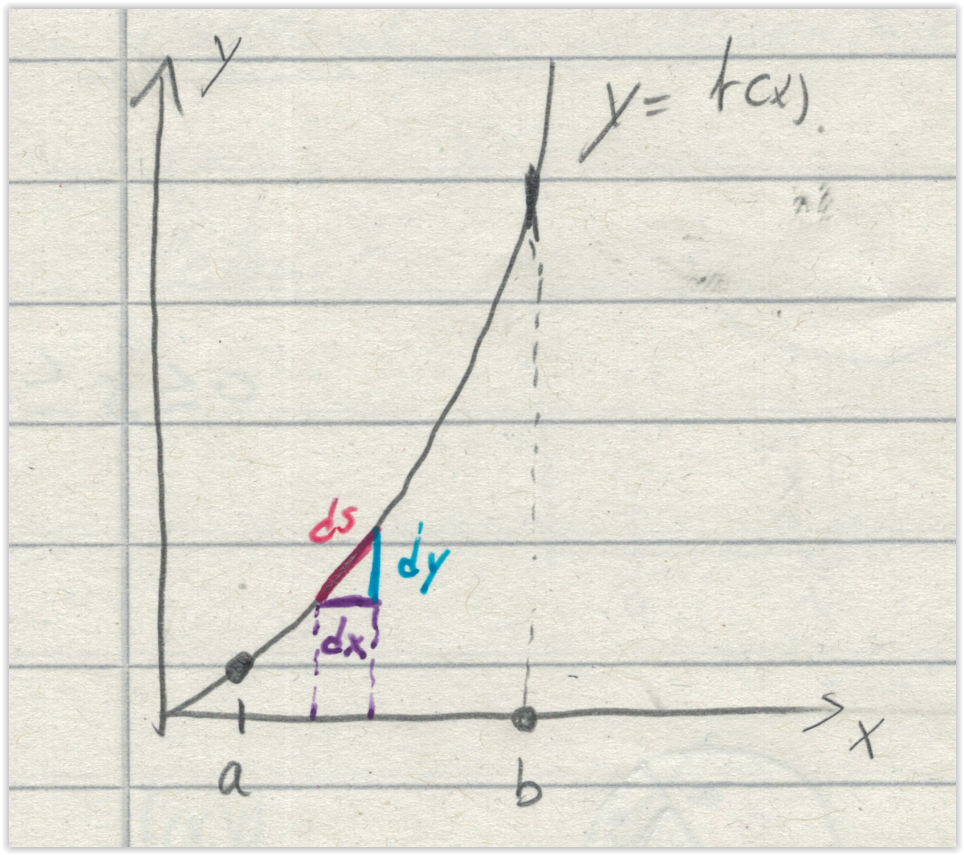
\includegraphics[width=0.4\linewidth]{./img/kurvenlaenge.png}
			  \caption{Kurvenlänge}
			  \label{fig:lkurvenlaenge}
      \end{figure}
	  \end{bem}
	  
	  \subsubsection{Flächen geschlossener ebener Kurven}
	  \begin{equation}
	    F(c) = \frac{1}{2} \int\limits_a^b \big|\big(x(t)\dot{y}(t) - y(t)\dot{x}(t)\big)\big|dt
	  \end{equation}
  \subsection{Wegintegrale}
	  \subsubsection{Wegintegral erster Art}
	  \begin{definition}
	    Das Wegintegral erster Art ist definiert durch:
	    \begin{equation}
	      \int\limits_c \varrho \; dx = \int\limits_x \varrho \; ds = \int\limits_a^b \varrho(c(t)) \quad || \dot{c}(t)|| dt \label{eq:wegintegral_1}
	    \end{equation}
	  \end{definition}
	  \begin{bem}
	    Aus \eqref{fig:wegintegral_erster_2} geht
	    \begin{equation*}
	      ds = \sqrt{dx^2 + dy^2}
	    \end{equation*}
	    hervor. Damit folgt:
	    \begin{align*}
	      ds &= \sqrt{dx^2 + dy^2} = \frac{dt}{dt}  \sqrt{dx^2 + dy^2} = \frac{1}{dt} \sqrt{dx^2 + dy^2}dt \\
	      &=  \sqrt{\frac{1}{dt^2}(dx^2 + dy^2)} =  \sqrt{\left(\frac{dx}{dt}\right)^2 + \left(\frac{dy}{dt}\right)^2}
	    \end{align*}
	    Überträgt man das bekannte Integral aus dem $\R^2$, das mit $\int\limits_a^b f(x) dx$ gegeben ist, und  obigen Zusammenhang ein, so erhält man:
	    \begin{align*}
	      \int\limits_{t=a}^{t=b} f(x,y) ds = \int\limits_{t=a}^{t=b} f(x,y) \sqrt{dx^2 + dy^2}\\
	      = \int\limits_{t=a}^{t=b} \underbrace{f(x(t),y(t))}_{\text{Höhe}} \underbrace{\sqrt{\left(\frac{dx}{dt}\right)^2 + \left(\frac{dy}{dt}\right))^2} dt}_{ds}
	    \end{align*}
	  \end{bem}
	  \begin{figure}[H] 
		\centering
		\begin{minipage}{.5\textwidth}
		  \centering
		  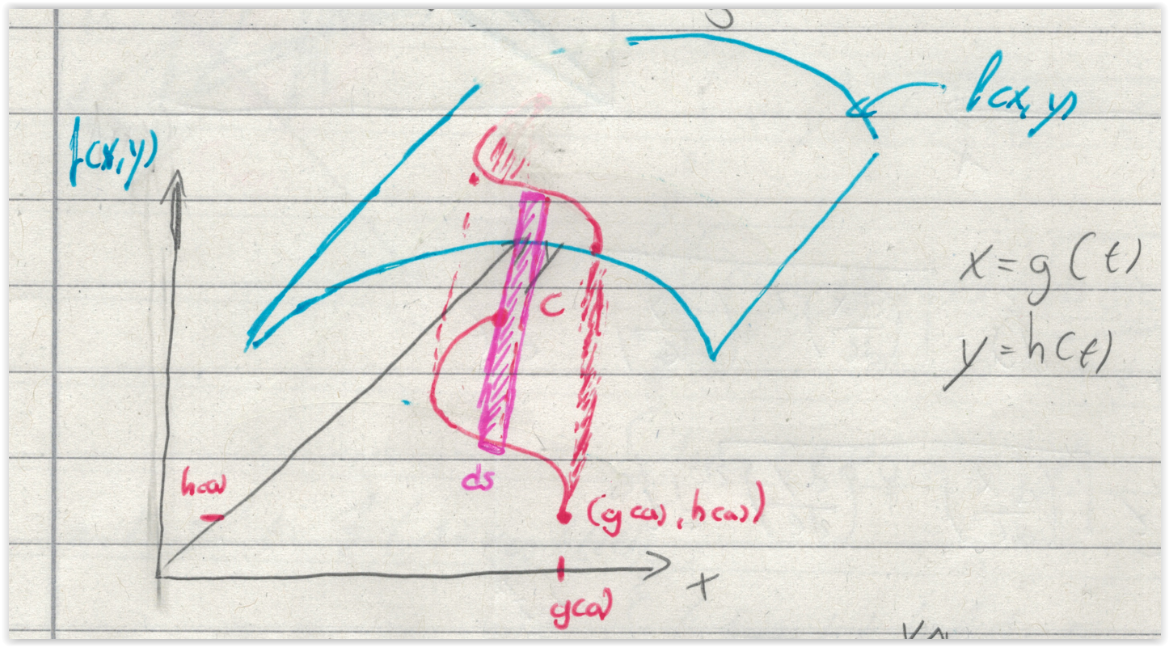
\includegraphics[width=0.9\linewidth]{./img/wegintegral_erster_1.png}
		  \caption{Graphische Interpretation}
		  \label{fig:wegintegral_erster_1}
		\end{minipage}%
		\begin{minipage}{.5\textwidth}
		  \centering
		  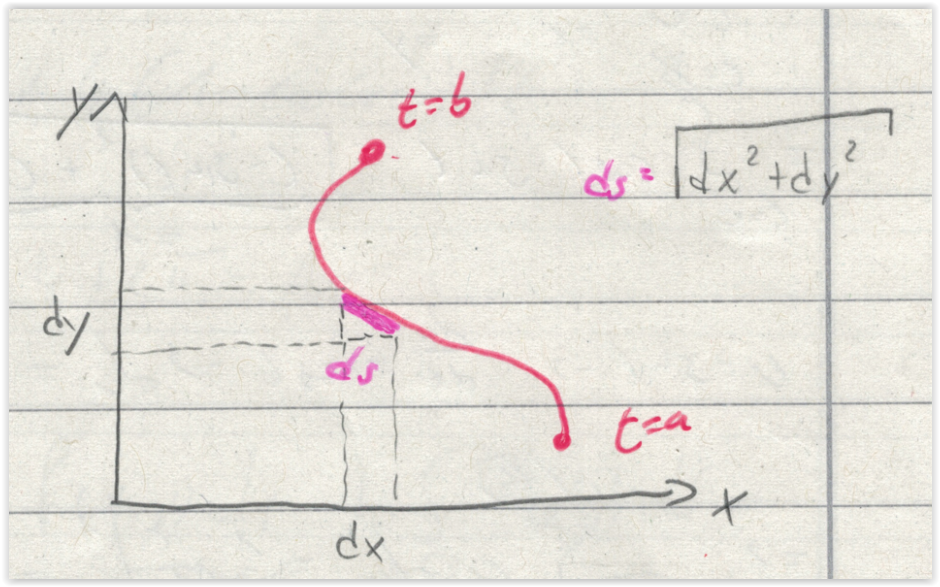
\includegraphics[width=0.8\linewidth]{./img/wegintegral_erster_2.png}
		  \caption{Interpretation von \protect\eqref{eq:wegintegral_1}}
		  \label{fig:wegintegral_erster_2}
		\end{minipage}
		\end{figure}
		\begin{bem}
			\begin{itemize}
			  \item[a) ] Integrale sind unabhängig von der gewählten Parametrisierung.
			  \item[b) ] Falls $c$ geschlossen ist so schreibt man 
				  \begin{equation}
				    \oint\limits_c \varrho \; ds
				  \end{equation}
			\end{itemize}
		\end{bem}
		\subsubsection{Wegintegrale zweiter Art}
		\begin{definition}
		  Sei $f: D\rightarrow \R^d$ ein stetiges Vektorfreld mit $D\subset \R^d$ und sei $c:[a,b] \rightarrow D$ eine stückweise $C^1$-Kurve, dann heißt 
		  \begin{equation}
		    \int\limits_c <f(x), dx> = \int\limits_a^b <f\left(c(t)\right), \dot{c}(t)>dt
		  \end{equation}
		  das Wegintegral 2-ter Art. Falls $c$ geschlossen ist schreibt man
		  \begin{equation}
		    \oint\limits_c <f(x), dx>
		  \end{equation}
		\end{definition}
		\begin{bem}
		  Das Wegintegral ist unabhängig von der gewählten Parametrisierung.
		\end{bem}
		\begin{bem}
		  Eine Alternative ältere Schreibweise ist
		  \begin{equation*}
		    \int\limits_c <f(X),dX>
		  \end{equation*}
		  Achtung, es handelt sich nur um eine Schreibweise. Nicht das Skalarprodukt aus $f(X)$ und $dX$ bilden!
		\end{bem}
		\begin{definition}
  		Ein stetiges Vektorfeld $f$ heißt wirbelfrei, falls die Kurvenintegrale längs aller stückweise stetig diffbaren Kurven verschwinden, d.h.
  		\begin{equation}
  		  \oint\limits_c <f(x), dx> = 0
  		\end{equation}
  		gilt.
		\end{definition}
		Als Konsequenz daraus folgt die Wegunabhängigkeit der Kurvenintegrale für den Fall das $f$ wirbelfrei ist. Das heißt, ist $f$ wirbelfrei, so gilt:
		\begin{equation}
		  \int\limits_{c_1} <f(x),dx> = \int\limits_{c_2} <f(x),dx>
		\end{equation}
		für beliebige Wege $c_1$ und $c_2$ mit gleichen Anfangs- und Endpunkten.
		\begin{definition}
		  Eine Teilmenge $D \subset \R^d$ heißt (weg)-zusammenhängend, falls je zwei Punkte $x,y \in D$ durch eine stückweise $C^1$-Kurve in $D$ verbunden werden können.
		  \begin{figure}[H] 
			  \centering
			  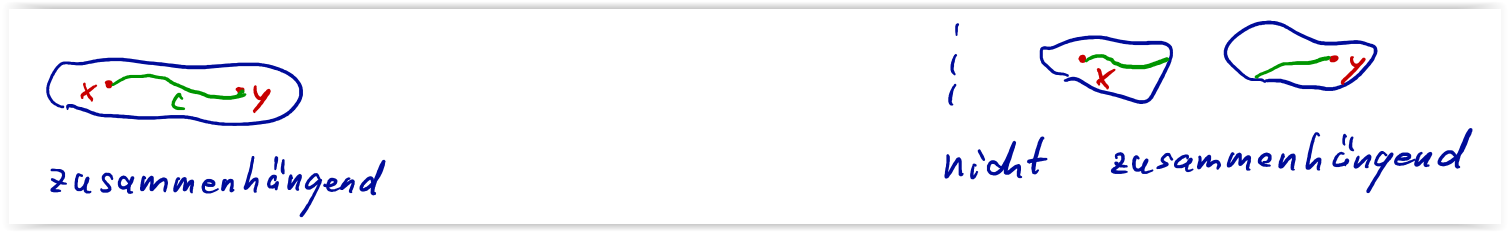
\includegraphics[width=0.8\linewidth]{./img/zusammenhaengend.png}
			  \caption{Visualisierung zusammenhängend \protect\cite{HM12}}
			  \label{fig:zusammenhängend}
		  \end{figure}
		\end{definition}
		\subsubsection{Potential}
	  \begin{definition}
	    Sei $f:D\rightarrow \R^d$ ein Vektorfeld auf $D\subset \R^d$. Wir sagen $f$ ist ein gradientenfeld, falls es eine skalare $C^1$-Funktion $\varphi: D\rightarrow\R$ gibt, mit 
	    \begin{equation}
	    \nabla \varphi(x) = f(x)
	    \end{equation}
	    $\varphi$ heißt das Potential von $f$.
	  \end{definition}
    \begin{satz}
      Sei $D \subset \R^n$ offen und zusammenhängend und $f$ ein stetiges Vektorfeld auf $D$. 
      \begin{itemize}
        \item[a) ] Besitzt $f$ ein Potential $\varphi$, so gilt für alle stückweisen $C^1$-Kurven $c$, dass 
        \begin{equation}
          \int\limits_c <f(x),dx> = \varphi(c(b)) - \varphi(c(a))
        \end{equation}
        wobei $c:[a,b]\rightarrow \R^d$. D.h. das Wegintegral ist damit wegunabhängig und $f$ wirbelfrei.
        \item[b) ] Ist $f$ wirbelfrei, so besitzt $f$ ein Potential $\varphi$ mit der Darstellung 
        \begin{equation}
          \varphi(x) = \int\limits_{c_x} f(\tilde{x}),d\tilde{x}>
        \end{equation}
        wobei $c_x$ ein Weg nach $x$ mit fest gewähltem Startpunkt $x^*$ sein soll.
      \end{itemize}
    \end{satz}	  
	  \subsubsubsection{Berechnung von Potentialen}
	  Die notwendige (aber nicht hinreichende) Bedingung für die Existenz eines Potentials ist:
	  \begin{equation}
	    rot(\nabla \varphi) = 0 \Rightarrow rot(f) = 0 \Rightarrow Potential\;ex.  
	  \end{equation}
	  \begin{definition}
	    Ein Gebiet $G$ heißt einfach zusammenhängend, falls jeder geschlossene Weg in $G$ auf einen Punkt im Gebiet zusammen gezogen werden kann.
	    \begin{figure}[H] 
			  \centering
			  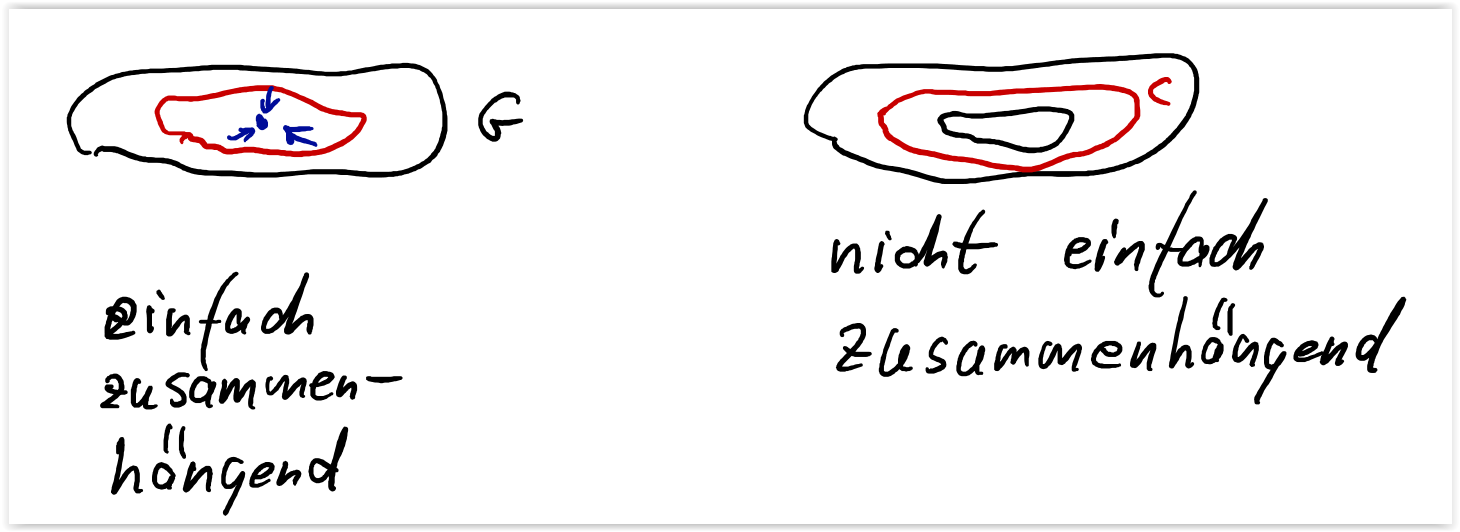
\includegraphics[width=0.8\linewidth]{./img/einfach_zusammenhaengend.png}
			  \caption{Visualisierung einfach zusammenhängend \protect\cite{HM12}}
			  \label{fig:einfach_zusammenhängend}
		  \end{figure}
	  \end{definition}
	  
  \newpage